\chapter{Gráficas y Superficies}

La teoría de gráficas y el estudio de superficies constituyen dos áreas fundamentales de las matemáticas que, en principio, podrían parecer independientes. Sin embargo, ambas se encuentran estrechamente relacionadas cuando una superficie se describe mediante triangulaciones y complejos simpliciales. Esta relación permite traducir ciertos problemas topológicos al lenguaje combinatorio de las gráficas, lo cual resulta especialmente útil para el desarrollo de métodos algorítmicos orientados al análisis y clasificación de superficies.
En el contexto de esta tesis, dicha conexión adquiere un papel central, ya que el objetivo principal es desarrollar un algoritmo de optimización de gráficas para el estudio del género de superficies asociadas a nudos. Para ello, es necesario establecer primero las nociones básicas que permiten pasar de un objeto geométrico o topológico, como una superficie, a una representación discreta mediante vértices y aristas. Esta representación facilita el uso de herramientas provenientes de la teoría de gráficas, así como su posterior incorporación en modelos computacionales y redes neuronales gráficas.
De manera general, una \textbf{gráfica} puede entenderse como un conjunto de \textbf{vértices} conectados mediante \textbf{aristas} \cite{haru}. Por otro lado, una \textbf{superficie} es un objeto que localmente se comporta como el plano ($\mathbb{R}^2$) \cite{pressley}, como ocurre con ejemplos clásicos tales como la esfera o el toro. A su vez, un \textbf{complejo simplicial} puede describirse como una colección de vértices junto con ciertos subconjuntos de estos, llamados \textbf{símplices}, que satisfacen propiedades específicas \cite{minian_complejos_simpliciales_poliedros}. Estas tres nociones serán desarrolladas con mayor precisión a lo largo del capítulo.
La importancia de los complejos simpliciales radica en que permiten triangular superficies y, a partir de dicha triangulación, inducir una gráfica sobre ellas. Esta representación discreta facilita el estudio de propiedades topológicas mediante herramientas combinatorias y resulta especialmente relevante para esta tesis, ya que permite analizar superficies asociadas a nudos de Lissajous y aplicar algoritmos de optimización orientados al estudio de su género. Por ello, este capítulo introduce los conceptos fundamentales de superficies, complejos simpliciales, triangulaciones y teoría de gráficas, los cuales servirán como base para justificar y construir el algoritmo propuesto en capítulos posteriores.
La primera parte del capítulo, dedicada a conceptos topológicos y complejos simpliciales, se basa principalmente en los textos de \cite{munkres_topology_2000}, \cite{prieto_topologia_2003} y \cite{minian_complejos_simpliciales_poliedros}. La segunda parte, enfocada en definiciones, propiedades y algoritmos de teoría de gráficas, toma como referencia los textos de \cite{haru}, \cite{diestel} y \cite{pressley}. A lo largo del capítulo, las definiciones se presentarán de manera formal y rigurosa, acompañadas de comentarios explicativos que permitan interpretar su significado y su utilidad dentro del desarrollo general de la tesis.

\section{Superficies}
Para comprender adecuadamente el objeto de estudio que se construye a lo largo de esta tesis, comenzaremos por introducir uno de los conceptos fundamentales que utilizaremos desde el inicio: el de superficie. Sin embargo, para poder definirlo con rigor, es necesario establecer previamente una serie de conceptos sobre los cuales se apoya esta definición.
Algunas definiciones no se mencionarán en este capítulo ya que podría considerarse que el lector está familiarizadas con ellas, pero para mantenerlas en contexto se incluyen en el apéndice \ref{ap:basicas}.

\subsection{Espacio Topológico}

De manera intuitiva, un \textbf{espacio topológico} puede entenderse como un conjunto al que se le ha asignado una colección especial de subconjuntos, llamados \textbf{conjuntos abiertos}. Esta colección no es arbitraria, pues debe satisfacer condiciones específicas que permiten estudiar nociones como continuidad, vecindad y proximidad, sin necesidad de recurrir a una medida de distancia. Formalmente, dicha colección debe contener al conjunto vacío y al conjunto total, ser cerrada bajo uniones arbitrarias y bajo intersecciones finitas.

\begin{definition}[Espacio topológico]

Sea $X$ un conjunto. Una \textbf{topología} sobre $X$ es una colección $\mathcal{T}$ de subconjuntos de $X$ que satisface los siguientes axiomas:

\begin{enumerate}
    \item $\emptyset \in \mathcal{T}$ y $X \in \mathcal{T}$.
    \item Si $\{U_i\}_{i \in I}$ es una familia arbitraria de elementos de $\mathcal{T}$, entonces
    \[
        \bigcup_{i \in I} U_i \in \mathcal{T}.
    \]

    \item Si \(U_1,\ldots,U_n \in \mathcal{T}\), entonces
    \[
        \bigcap_{j=1}^{n} U_j \in \mathcal{T}.
    \]
\end{enumerate}

A la pareja $(X,\mathcal{T})$ se le denomina \textbf{espacio topológico}, y a los elementos de $\mathcal{T}$ se les llama \textbf{conjuntos abiertos}.
\end{definition}
La presente definición nos proporciona un marco general para trabajar con nociones geométricas de manera más flexible, lo cual resulta útil en contextos que, a simple vista, podrían parecer triviales.
\\A continuación, presentaremos un ejemplo que, a pesar de su simplicidad aparente, ilustra de una manera adecuada la estructura de un espacio topológico y revela propiedades interesantes.

\begin{example}
    Sea $X$ un conjunto de dos elementos $X = \{x,y\}$, podemos definir una topología sobre este conjunto de la siguiente forma:
    \\Tomemos los conjuntos abiertos: $\mathcal{T} = \{X,\emptyset, \{x\} \}$
    \\Entonces observamos que:
    
    $\{x\} \cup X =X$, $\{x\} \cup \emptyset = \{x\}$,
    $X \cup \emptyset = X$, $\{x\} \cap X = \{x\}$,
    $\{x\} \cap \emptyset = \emptyset$, $X \cap \emptyset = \emptyset$
    
    Por tanto $(X,\mathcal{T})$ es un espacio topológico, en específico se le conoce como espacio topológico de Sierpiński.
    
\end{example}
Este espacio, aunque pequeño, nos muestra propiedades útiles en el estudio de conceptos como separación y continuidad, además su importancia radica en que sirve como el ejemplo más sencillo de un espacio no trivial que distingue entre puntos, y es frecuentemente utilizado como caso de prueba en demostraciones, en la caracterización de funciones continuas, y en demás propiedades.

Otro de los conceptos en el que nos auxiliaremos para construir y tratar las superficies trabajadas es el concepto de \textbf{conjunto cerrado}, el cual no es más que la contraparte de la definición de conjunto abierto. Notaremos que la relación entre ambos es directa: un conjunto cerrrado es aquel cuyo complemento es un conjunto abierto.
\begin{definition}[Conjunto cerrado]
    Sea $X$ un espacio topológico. Decimos que un subconjunto $A$ de $X$ es \textbf{cerrado} si el conjunto $X-A$ es abierto.   
\end{definition}

El siguiente ejemplo es bastante útil visualmente ya que se muestra explícitamente cómo se aplica la definición de conjunto cerrado en un caso concreto.

\begin{example}
    Sea $A = \{x \times y | x\geq 0 \hspace{5pt} e \hspace{5pt} y \geq 0\} \subset \mathbb{R}^2$,entonces el conjunto A es cerrado.
    \begin{proof}
        Observamos que el complemento de $A$ es:
         \[\{x \times y \hspace{5pt}| x < 0 , y \geq 0\} \cup \{x \times y \hspace{5pt} | x \geq, y <0 \} \cup \{x \times y  \hspace{5pt}| x<0 , y <0 \}\] es decir \[\{x \times y \hspace{5pt}| x <0 , y \in \mathbb{R}\} \cup \{x \times y\hspace{5pt} | x \in \mathbb{R} \times y < 0\}\] lo cual es equivalente a  \[(- \infty , 0) \times \mathbb{R} \cup \mathbb{R} \times (0, \infty)\] , como cada uno de ellos es abierto y la unión de abiertos es abierta, entonces el complemento de $A$ es abierto y por lo tanto $A$ es un conjunto cerrado.
    \end{proof}

\end{example}

\begin{figure}[H]
    \centering
    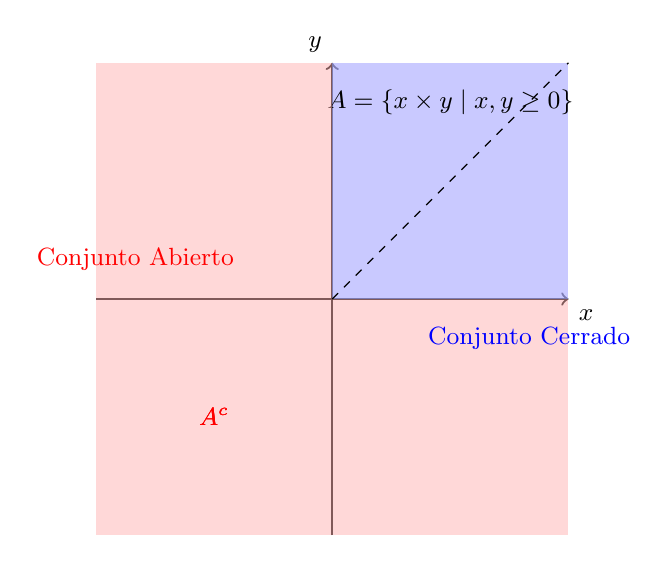
\begin{tikzpicture}
        % Ejes coordenados
        \draw[thick,->] (-3,0) -- (3,0) node[anchor=north west] {\small $x$};
        \draw[thick,->] (0,-3) -- (0,3) node[anchor=south east] {\small $y$};
    
        % Región del conjunto A (x*y con x,y >= 0)
        \fill[blue!30,opacity=0.7] (0,0) rectangle (3,3);
        \node at (1.5,2.5) {\small $A = \{x \times y \mid x, y \geq 0\}$};
    
        % Región del complemento A^c (parte negativa)
        \fill[red!30,opacity=0.5] (-3,-3) rectangle (0,0);
        \node[red] at (-1.5,-1.5) {\small $A^c$};
        \fill[red!30,opacity=0.5] (-3,3) rectangle (0,0);
        \node[red] at (-1.5,-1.5) {\small $A^c$};
        \fill[red!30,opacity=0.5] (3,-3) rectangle (0,0);
        \node[red] at (-1.5,-1.5) {\small $A^c$};
    
        % Etiquetas
        \node[blue] at (2.5,-0.5) {\small Conjunto Cerrado};
        \node[red] at (-2.5,0.5) {\small Conjunto Abierto};
    
        % Línea divisoria en x=0 e y=0
        \draw[dashed] (0,0) -- (3,3);
    \end{tikzpicture}
    \label{fig:cerrado}
    \caption{Ilustración del suconjunto $A$}
    
\end{figure}

De la mano de las definiciones de conjuntos abierto y cerrados podemos entender que existe el uso de estos conceptos para definir y establecer regiones sobre un espacio topológico. Notaremos que a partir de las definiciones de interior, cerradura y frontera podemos llegar de forma natural a la consideración de un axioma para espacios topológicos, el cual abordaremos más adelante.

\begin{definition}[Interior de un conjunto]
    Sea $X$ un espacio topológico y $A$ un subconjunto de $X$.
    El \textbf{interior} de $A$ se define como la unión de todos los conjuntos abiertos contenidos en $A$, es decir \[
    Int A = \displaystyle \bigcup_{i \in \mathcal{I}} A_i \hspace{5pt} | \hspace{5pt} A_i \subset A\] con $A_i$ abierto para $i \in \mathcal{I}$.   
\end{definition}

\begin{proposition}
    Sea $X$ un espacio topológico y $A$ un conjunto abierto.
    Entonces $A$ es abierto en $X$ si y sólo si $IntA = A$
\end{proposition}

\begin{definition}[Cerradura de un conjunto]
    Sea $X$ un espacio topológico y $A$ un subconjunto de $X$.
    La \textbf{cerradura} de $A$ se define como la intersección de todos los conjuntos cerrados que conitienen a $A$, es decir \[
    \bar{A} = \displaystyle \bigcap_{i \in \mathcal{I}} A_i \hspace{5pt} | \hspace{5pt} A \subset A_i\] con $A_i$ cerrado para $i \in \mathcal{I}$.
\end{definition}
\begin{proposition}
    Sea $X$ un espacio topológico y $A$ un conjunto cerrado.
    Entonces $A$ es cerrado en $X$ si y sólo si $\bar{A} = A$
\end{proposition}

\begin{definition}[Frontera de un conjunto]
    Sea $X$ un espacio topológico y $A$ un subconjunto de $X$. Un punto $x \in \bar{A} \cap \overline{X-A} $ se denomina \textbf{punto frontera} de $A$; al conjunto  $\bar{A} \cap \overline{X-A}$ se le llama \textbf{frontera} de $A$.
    
\end{definition}

\subsection{Espacio de Hausdorff}

Notemos que, en cierto modo, las definiciones de la sección anterior nos hablan del comportamiento de los puntos respecto a un conjunto. Con la noción de \textbf{interior} podemos describir cuándo un punto "pertenece completamente" a la región; la \textbf{cerradura} nos indica cuándo un punto está lo suficientemente "cerca" de ella; y la \textbf{frontera} señala que un punto está justo "en el límite" de dicho conjunto. A partir de estas ideas surge de forma natural la condición que define un \textbf{espacio de Hausdorff}: que dos puntos distintos "no se tocan", es decir, que existen entornos abiertos disjuntos alrededor de cada uno, cuyas cerraduras tampoco se intersecan. En consecuencia, sus interiores quedan totalmente separados.
Este requisito cobra especial relevancia al pasar de ejemplos familiares, como $\mathbb{R}$ o $\mathbb{R}^2$, donde cada conjunto puntual $\{x_0\}$ es automáticamente cerrado, a topologías más generales en las que ese hecho ya no se cumple. Para evitar estudiar espacios en los que los puntos no puedan separarse nítidamente introducimos la definición de espacios de Hausdorff. 
En el contexto de esta tesis, este criterio nos permitirá centrar nuestro análisis exclusivamente en objetos que satisfagan dicha condición de separación.

\begin{definition}(Espacio de Hausdorff)
    \\Sea $(X,\mathcal{A})$ un espacio topológico.Se dice que $X$  es un \textbf{Espacio de Hausdorf}, si para cada par $x_1, x_2$ de puntos distintos de $X$, existen vecindades $U_1,U_2$ de $x_1,x_2$ respectivamente, que son ajenas. Es decir $U_1 \cap U_2 = \emptyset$
\end{definition}

\begin{example}
    Sea $X = \mathbb{R}$ y definamos la topología dada por el conjunto $\mathcal{B} = \{(a,b) | \hspace{5pt} 0 \in (a,b) \subset \mathbb{R} \}$.
    Tomemos dos puntos distintos arbitrarios, es decir $x \neq y \in X$, entonces queremos ver si existen dos vecindades $U,V$ de $x,y$ tales que $U \cap V = \emptyset$. Pero por la construcción de $\mathcal{B}$, toda vecindad contiene al punto 0, por tanto $U \cap V \neq \emptyset$ y por lo tanto no es de Hausdorf.
    
\end{example}

\begin{teorema}
    Sea $X$ un espacio topológico de Hausdorf. Sea $U$ un conjunto con un número finito de puntos. Entonces $U$ es cerrado.
\end{teorema}

\begin{proof}
    Sean $x,x_0$ en $X$ tales que $x \neq x_0$. Como $X$ es de Hausdorf entonces existen vecindades $U,V$ tales que $U \cap V = \emptyset$.
    Cómo $U$ no interseca al conjunto ${x_0}$ entonces el punto $x$ no puede pertenecer a la cerradura del conjunto ${x_0}$.Como consecuencia $\overline{\{x_0\}} = {x_0}$, por lo tanto es cerrado.
\end{proof}

\subsection{Compacidad}
Otra de las propiedades importantes que necesitamos para entender los objetos centrales de este escrito, es el concepto de compacidad. 
De manera intuitiva podemos decir que un espacio es compacto si podemos "cubrirlo" por completo por conjuntos más pequeños pero que en la suma, den el espacio total.
Comencemos por definir en primera instancia a que nos referimos por "cubierta", específicamente a "cubierta abierta".

\begin{definition}(Cubierta abierta)
    \\Sea $X$ un espacio topológico, sea $\mathcal{A} = \{\mathcal{A}_i\}_{i \in \mathcal{I}}$ una familia de subconjuntos abiertos de $X$.
    \\Se dice que $\mathcal{A}$ es una \textbf{cubierta abierta} de $X$ si $X \subseteq \displaystyle \bigcup_{i \in \mathcal{I}} \{\mathcal{A}_i\} $
    
\end{definition}

\begin{definition}(Subcubierta finita)
    Sea $X$ un espacio topológico, sea $\mathcal{A}$ una cubierta abierta de $X$. 
    \\Decimos que $\mathcal{A}'$ es una subcubierta de $\mathcal{A}$ si $\mathcal{A}' \subset \mathcal{A}$, en particular si $\mathcal{A}'$ es finito, entonces es una \textbf{subcubierta finita}.
    
\end{definition}
Por último buscamos cubrir en su totalidad de manera controlada y finita por estos objetos que definimos anteriormente, de esta forma la defición de espacio compacto queda como sigue:

\begin{definition}(Espacio Compacto)
    \\Sea $X$ un espacio topológico, se dice que $X$ es \textbf{compacto} si de cada cubierta abierta podemos extraer una subcubierta finita de $X$.
\end{definition}

\begin{example}
    Sea $X = \{0\} \cup \{ \frac{1}{n} \hspace{5pt} | \hspace{5pt} n \in \mathbb{Z}_{+} \}$ un subespacio de $\mathbb{R}$.
    \\Demostraremos a continuación que el espacio $X$ es un espacio compacto:
    \begin{proof}
        Sea $\{\mathcal{A}_{\alpha}\}$ una cubierta abierta de $X$, es decir $X \subseteq \displaystyle \bigcup_{\alpha} \mathcal{A}_{\alpha}$.
        \\Como $0 \in X$ y $\{\mathcal{A}_{\alpha}\}$ es cubierta abierta, entonces existe un entorno abierto $\mathcal{A}_0$ que contiene a 0, es decir , existe $\epsilon > 0$ tal que $(-\epsilon, \epsilon) \subseteq \mathcal{A}_0$.
        Notamos que, en particular existe un $N$ suficientemente grande tal que para todo $n>N$, se cumple que $\frac{1}{n} \in (-\epsilon,\epsilon)$, de ahí que los puntos de la forma $\frac{1}{N},\frac{1}{(N+1)},\frac{1}{(N+2)}, \dotsc $ están en $\mathcal{A}_0$, ahora los puntos restantes $1,2,\dotsc ,\frac{1}{N-1}$ notamos que son finitos y además están en algún $\mathcal{A}_{\alpha}$.Es decir están en una subcubierta finita.
        \\Por último notamos que la subcubierta finita de $X$ es de la forma $\mathcal{A}_0 \cup \mathcal{A}_{1} \cup \cdots \cup \mathcal{A}_{N-1}$ por tanto, $X$ es compacto.

    \end{proof}

\end{example}
\begin{figure}[ht]
    \centering
    \begin{center}
        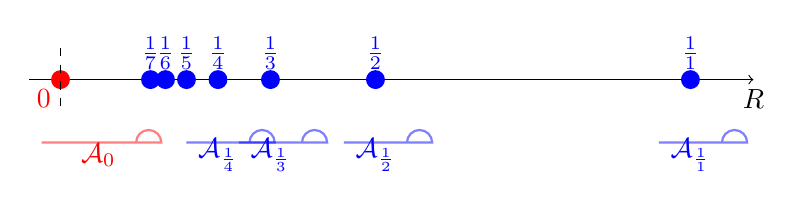
\begin{tikzpicture}[scale=8]
            \draw[->] (-0.05,0) -- (1.1,0) node[below] {$\mathbb{R}$};
            \filldraw[red] (0,0) circle (0.4pt) node[below left] {$0$};
    
            
            \foreach \n in {1,2,3,4,5,6,7} {
                \filldraw[blue] ({1/\n},0) circle (0.4pt) node[above] {$\frac{1}{\n}$};
            }
    
            % Indicador de la sucesión que converge a 0
            \draw[dashed] (0,0.05) -- (0,-0.05);
    
            % Entorno abierto alrededor de 0
            \draw[red,thick,opacity=0.5] (-0.03,-0.1) -- (0.12,-0.1) arc[start angle=180, end angle=0, radius=0.02] -- cycle;
            \node[red] at (0.06,-0.12) {$\mathcal{A}_0$};
    
            % Entornos abiertos para algunos puntos
            \foreach \n in {1,2,3,4} {
                \draw[blue,thick,opacity=0.5] ({1/\n - 0.05},-0.1) -- ({1/\n + 0.05},-0.1) arc[start angle=180, end angle=0, radius=0.02] -- cycle;
                \node[blue] at ({1/\n},-0.12) {$\mathcal{A}_{\frac{1}{\n}}$};
            }
        \end{tikzpicture}
    \end{center}
    \label{fig:compacto}
    \caption{Ilustración de la compacidad del espacio $X$}

\end{figure}
\begin{lemma}
    Sea $X$ un espacio topológico.Sea $Y$ un subspacio de $X$. Entonces $Y$ es compacto si, y sólo sí , cada cuberta de $Y$ por abiertos de $X$ contiene una subcolección finita que cubre a $Y$.
\end{lemma}

\begin{proof}
Supongamos primero que $Y$ es compacto y que $\mathcal{A} = \{A_{\alpha}\}_{\alpha \in J}$ es una cubierta de $Y$ por abiertos de $X$, entocnes la colección:

\[
\{A_{\alpha} \cap Y\ | \alpha \in J\}
\]
es una cubierta de $Y$ por conjuntos abiertos en $Y$; como $Y$ es compacto entonces existe una subcubierta abierta finita de la forma 
\[
\{A_{\alpha_1} \cap Y, \cdots , A_{\alpha_n} \cap Y\}
\]

\end{proof}
Notamos además que, existe una relación entre los espacios compactos y los espacios de Hausdorf que definimos anteriormente: 
\begin{teorema}
    Sea $X$ un espacio topológico de Hausdorf. Sea $Y$ un subespacio compacto de $X$, entonces $Y$ es cerrado.
\end{teorema}

\begin{proof}
    Sea $Y$ un subespacio compacto de un espacio topológico de Hausdorff $X$. Queremos mostrar que  $X-Y$ es abierto, y por tanto $Y$ será cerrado.

    Sea $x_0$ un punto en $X-Y$.Procederemos a demostrar que existe un entorno de $x_0$ que no interseca a $Y$. 

    Cómo $X$ es de Hausdorf, elegimos entornos disjuntos $U_{y}$ y $V_y$ de los puntos $x_0$ y $y$ respectivamente, para cada punto $y \in Y$.
    Ahora, notamos que la colección
    \[
    \{V_y | y \in Y \}
    \] es una cubierta de de $Y$ por abiertos de $X$, como $Y$ es compacto, entonces existe una subcolección finita de la forma $V = \{V_{y_1},\cdots , V_{y_n}\}$ que cubre a $Y$.
    Además notamos que el conjunto 
    \[
    U = \{ U_{y_1} \cap \cdots \cap U_{y_n} \}
    \] formado de tomar las intersecciones de los correspondientes entornos $x_0$ es disjunto con $V$. Ya que si $z \in V$ entonces $z \in V_{y_i}$ para algún $i$, por lo tanto $z \notin U_{y_i}$, y por tanto $z \notin U$. Así $U$ es un entorno de $x_0$ que no interseca a $Y$, lo que implica que $X-Y$ es abierto. Por tanto $Y$ es cerrado.
\end{proof}

\subsection{Espacios numerables}
Por últmo, definiremos otra de las propiedas que nos sirven como base para llegar a definir nuestro objetivo, la cual es la de \textbf{numerabilidad}. 
Esta propiedad nos permite establecer una relación entre los puntos de un espacio topológico y las vecindades que estos poseen. En particular, nos interesa saber si cada punto tiene una base de vecindades numerable, lo que nos permitirá trabajar con espacios más manejables y estructurados.

\begin{definition}(Base de vecindades)
    \\Sea $X$ un espacio topológico y $x \in X$. Decimos que una familia $\mathcal{B}_x$ de vecindades de $x$ es una \textbf{base de vecindades} de $x$ si para cualquier vecindad $U$ de $x$ existe una vecindad $V \in  \mathcal{B}_x$ tal que $V \subset U$
\end{definition}

\begin{definition}(Base numerable)
    Sea un espacio toplógico $X$. Se dice que $X$ tiene una base numerable en $x$ si existe una base de vecindades numerable.

\end{definition}


\begin{definition}(Primer axioma de numerabilidad)
    Sea $X$ un espacio topológico. Se dice que $X$ satisface el primer axioma de numerabilidad o que es 1-numerable, si cumple que, cada punto de $X$ tiene una base de vecindades numerable.
\end{definition}


\begin{definition}(Segundo axioma de numerabilidad)
    Sea $X$ un espacio topológico, se dice que $X$ satisface el segundo axioma de numerabilidad, o que es 2-numerable, si la topología $X$ admite una base numerable.
\end{definition}

\begin{example}
    Observamos que en la topología uniforme $\mathbb{R}^\omega$ satisface el primer axioma de numerabilidad por ser metrizable.Sin embargo no satisface el segundo. Para comprobar este hecho mostraremos que si $X$ es un espacio que tiene base numerable $\mathcal{B}$, entonces cualquies subespacio discreto $A$ de $X$ debe ser numerable. Elijamos para cada $a \in A$ un elemento $B_a$ de la base que interseque a $A$ unicamente en el punto a, si a y b son distintos de A , los conjuntos $B_a$ y $B_b$ son distintos , puesto que el primero contiene a $a$ y el segundo no. Se sigue que l aplicación $a \rightarrow B_a$ es una inyección de $A$ en $\mathcal{B}$, por lo que $A$ debe ser numerable.
    Ahora bien, el subespacio $A$ de $\mathbb{R}^\omega$ formado por todas las suscesiones de ceros y unos no es umerable y tiene la topologóa discreta porque $\bar{\rho}(a,b) = 1$ no tiene una base numerable.
\end{example}

\subsection{Variedades topológicas}

Para poder definir una superficie de forma rigurosa, es necesario establecer un contexto adecuado que nos permita trabajar con objetos que cumplan ciertas propiedades topológicas. En este sentido, las \textbf{variedades topológicas} son espacios que cumplen con condiciones específicas, como ser de Hausdorff y 2-numerables, lo que garantiza que cada punto tiene una base de vecindades numerable. Estas condiciones son fundamentales para asegurar que los puntos de la variedad se comporten de manera controlada y predecible, lo que facilita, en nuestro caso, el estudio de superficies. 

\begin{definition}(Variedad topológica)
    Un espacio topológico $X$, de Hausdorff, 2-numerable es una \textbf{variedad topológica} de dimensión n, también llamada n-variedad, si cada punto $x \in X$ tiene una vecindad homeomorfa a un abierto $U$ en la n-bola cerrada $\mathbb{B}^n$
\end{definition}

\begin{definition}
    (Superficie)\\
        Una $2-variedad$ $S$ es una superficie. Si es compacta y no tiene frontera se le llama \textbf{Superfice cerrada}
\end{definition}

\begin{example}

Sea $\mathrm{S}$ = $\{(x,y,z) \in \mathbb{R}^3 | z = x^2 - y^2 \}$
Demostraremos que $\mathrm{S}$ es una superficie, entonces , tenemos que demostrar que para cada punto $p \in \mathrm{S}$ existen conjuntos, $U \in \mathbb{R}^2$, $W \in \mathbb{R}^3$ abiertos tal que $p \in W \cap S$ y que existe $h: S\cap W \subset \mathbb{R}^3 \rightarrow U \subset \mathbb{R}^2$ tal que $h$ es un homeomorfismo.

\begin{proof}
    Sea $p = (x_0,y_o,z_0) \in S$ entonces por definición $ z_0 = x_0^2 - y_0^2$, por otro lado definimos a $W \subset \mathbb{R}^3$ como la bola abierta centrada en $p$ de radio $r$ $\mathcal{B}_p(r)$ y a $U \subset \mathbb{R}^2$ como la vecindad alrededor de $(x_0,y_0)$, $V(x_0,y_0)$.\\
    Definamos ahora la función $\Pi: \mathrm{S}\cap W \rightarrow U$ dada por:

    \[
    \Pi(x,y,x) = (x,y)
    \]
    Es decir la función proyección restringida a $\mathrm{S}\cap W$, ahora notemos lo siguiente:

    \begin{itemize}
        \item $\Pi$ es una función continua ya que es la restricción de la función proyección que es continua en $\mathbb{R}^3$.
        \item $\Pi$ es inyectiva pues, dado $u=(x_1,y_1,z_1),w=(x_2,y_2,z_2) \in S\cap W$ tenemos que :
        \begin{align*}
        \Pi(x_1,y_1,z_1) &= \Pi(x_2,y_2,z_2) \Rightarrow \\
        (x_1,y_1) &= (x_2,y_2) \Rightarrow \\
        x_1 = x_2 &, y_1 = y_2
        \end{align*}
        Por otro lado como $u,w \in S$ entonces:
        \begin{align*}
            z_1 = x_1^2 - y_1^2 = x_2^2 - y_2^2 = z_2
        \end{align*}
        Es decir :
        \begin{align*}
            u = (x_1,y_1,z_1) = (x_2,y_2,z_2) = w
        \end{align*}
        Por tanto $\Pi$ es inyectiva.
        \item Sea $(x,y) \in U$ entonces notamos que existe un punto en $p \in S \cap W$ dado por $p = (x,y,x^2-y^2)$ por tanto $\Pi$ es sobreyectiva.
        \item Notamos que $\Pi^{-1}$ está dada por $\pi^{-1}(x,y) = (x,y,x^2-y^2)$, como las componentes $x,y$ son continuas y $x^2 - y^2$ es una combinación lineal de componentes continuas entonces $\Pi ^{-1}(x,y)=(x,y,x^2 - y^2)$ es continua
    \end{itemize}
    Por tanto $\Pi$ es un homeomorfismo y por tanto $S \cap W$ es homeomorfo a $U$ y por lo tanto $S$ es una superficie.
\end{proof}


\begin{figure}[ht]
	\centering
    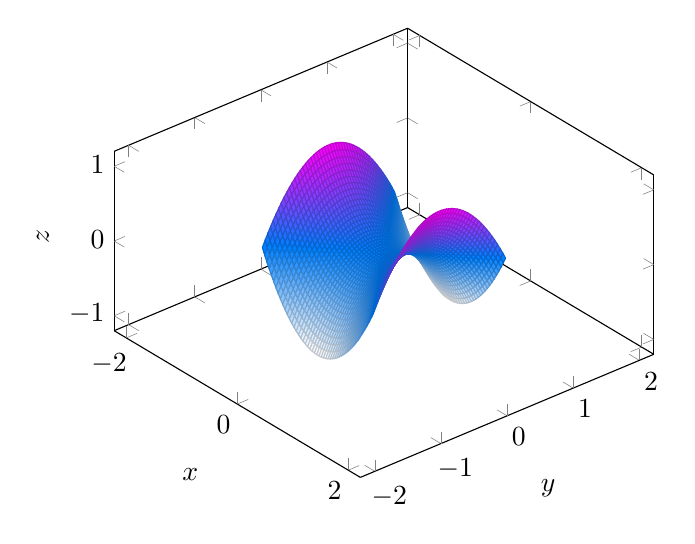
\begin{tikzpicture}
    \begin{axis}[
        view={50}{30}, % Ángulo de visión
        axis equal,
        colormap/cool,
        xlabel={$x$},
        ylabel={$y$},
        zlabel={$z$},
    ]
    \addplot3[surf, samples=50, domain=-1:1, y domain=-1:1] 
        {x^2 - y^2}; % Ecuación de la silla de montar
    \end{axis}

\end{tikzpicture}
    \label{fig:silla}
    \caption{Ejemplo de superficie en $\mathbb{R}^3$ comúnmente conocida como "Silla de Montar"}
\end{figure}


\end{example}

\subsection{Complejos simpliciales y triangulaciones}
Habiendo establecido una definición rigurosa de superficie, resulta natural preguntarse cómo representar estos objetos mediante estructuras discretas que sean más adecuadas para su análisis computacional. En este sentido, los \textbf{complejos simpliciales} proporcionan una herramienta muy útil para construir triangulaciones de superficies, permitiendo describirlas a partir de vértices y aristas. Notamos así que, los complejos simpliciales sirven como puente entre la geometría continua de las superficies y las herramientas combinatorias y algorítmicas que se utilizarán posteriormente para optimizar gráficas y estudiar el género de estos objetos.

\begin{definition}[Complejo simplicial]
Sea $V$ un conjunto finito cuyos elementos llamaremos \textbf{vértices}. Un \textbf{complejo simplicial} sobre $V$ es una colección $\mathcal{K}$ de subconjuntos no vacíos de $V$, llamados \textbf{símplices}, que satisface las siguientes propiedades:
    \begin{enumerate}
        \item Para todo vértice $v \in V$, el conjunto ${v}$ pertenece a $\mathcal{K}$.
        \item Si $\sigma \in \mathcal{K}$ y $\tau \subseteq \sigma$ con $\tau \neq \emptyset$, entonces $\tau \in \mathcal{K}$.
    \end{enumerate}
\end{definition}
Es decir, si un conjunto de vértices pertenece al complejo simplicial, entonces todos sus subconjuntos no vacíos también pertenecen al complejo. A los subconjuntos de un símplice se les llama \textbf{caras}.

De esta forma los complejos simpliciales permiten representar objetos geométricos mediante piezas simples. En particular, una superficie puede describirse a partir de una triangulación formada por vértices, aristas y triángulos. Y así esta representación discreta permite asociar una gráfica a la superficie al considerar sus vértices y aristas, lo cual facilita el uso de herramientas combinatorias y algoritmos de optimización.

\begin{figure}[H]
    \centering
    
    \begin{subfigure}[t]{0.32\textwidth}
        \centering
        
\includegraphics[width=\textwidth]{simplice_1.png}
        \caption{Complejo 1-simplicial.}
    \end{subfigure}
    \hfill
    \begin{subfigure}[t]{0.32\textwidth}
        \centering
        
\includegraphics[width=\textwidth]{simplice_2.png}
        \caption{Complejo 2-simplicial.}
    \end{subfigure}
    \hfill
    \begin{subfigure}[t]{0.32\textwidth}
        \centering
        
\includegraphics[width=\textwidth]{simplice_3.png}
        \caption{Complejo 3-simplicial.}
    \end{subfigure}
    
    \caption{Ejemplos de complejos simpliciales.}
    \label{fig:complejos_simpliciales}
\end{figure}


\section{Gráficas}

A partir de las definiciones previas, es posible introducir nuevos objetos que servirán como base para la caracterización formal de las superficies de interés. De este modo, comenzaremos definiendo las \textbf{gráficas}, que son estructuras matemáticas compuestas por vértices y aristas. Estas gráficas nos permitirán representar las superficies de manera más manejable y eficiente, facilitando su estudio y análisis. En particular, al considerar la triangulación de una superficie, cada 1-símplice puede ser representado como una gráfica, donde los vértices corresponden a los vértices del triángulo y las aristas a sus lados. Dada la naturaleza de la construcción de las superficies, estas gráficas serán simples, es decir, no tendrán bucles ni aristas múltiples. A continuación, se presentarán las definiciones y propiedades fundamentales de las gráficas simples, que servirán como base para el desarrollo posterior de la teoría.

\subsection{Gráficas simples y propiedades básicas}

\begin{definition}[Gráfica simple] 
Una gráfica simple $G$ está definida por un par ordenado $G = (V,E)$, donde V es un conjunto cuyos elementos son llamados vértices (o nodos) de la gráfica y E un conjunto cuyos elementos son las aristas de la gráfica. 
\end{definition}

\noindent Regularmente denotamos a $V$ y $E$ como $V(G)$ y $E(G)$ que hacen referencia a la gráfica G, entonces $G=(V(G),E(G))$
Definimos a $E$ como:
\begin{center}
$E(V)$ = $\{\{u,v\} | u,v \in V, u \neq v \}$
\end{center}
Usualmente denotamos al par $\{u,v\}$ simplemente como $uv$.

Derivado de la definición anterior, podemos establecer algunas propiedadesm que nos permitirán caracterizar y analizar los objetos de estudio de manera más precisa. Estas propiedades incluyen el orden y tamaño de la gráfica, así como las relaciones entre los vértices y aristas.

\begin{definition}[Orden y tamaño] 
Para una gráfica $G$ , tenemos que:
\begin{enumerate}
    \item $\nu_{G}$ = $|\mathbf{V(G)}|$ es llamado el orden de $G$.
    \item $\varepsilon_{G}$ = $|\mathbf{E(G)}|$ es llamado  el tamaño de $G$.
    \item Para cada arista $e = uv \in E$ los vértices $u$ y $v$ son llamados extremos de la arista.
    \item Los vértices $u$ y $v$ son adyacentes o vecinos si $e = uv \in E$.
    \item Dos aristas $e_1 = uv$ y $e_2 = uw$ tienen un extremo común, entonces son adyacentes entre sí.
\end{enumerate}
\end{definition}

\begin{figure}[H]
    \centering
    \begin{tikzpicture}[
        scale=0.9,
        every node/.style={
            circle,
            draw=black,
            fill=white,
            thick,
            minimum size=8mm,
            inner sep=0pt,
            font=\small
        }
    ]
    
    % Vértices
    \node[label=above:$v_1$] (n1) at (1,10) {};
    \node[label=above left:$v_2$] (n2) at (4,8) {};
    \node[label=above:$v_3$] (n3) at (8,9) {};
    \node[label=above right:$v_4$] (n4) at (11,8) {};
    \node[label=below right:$v_5$] (n5) at (9,6) {};
    \node[label=below left:$v_6$] (n6) at (5,5) {};

    % Aristas
    \draw[thick] (n1) -- (n2);
    \draw[thick] (n2) -- (n3);
    \draw[thick] (n3) -- (n4);
    \draw[thick] (n4) -- (n5);
    \draw[thick] (n5) -- (n6);
    \draw[thick] (n6) -- (n2);
    \draw[thick] (n6) -- (n3);

    \end{tikzpicture}
    \caption{Ejemplo de gráfica simple $G$.}
    \label{fig:G}
\end{figure}

\begin{flushleft}

En la figura \ref{fig:G} podemos observar que $\nu_{G}$ = 6, $\varepsilon_{G}$ =7, los extremos de la arista $ab$ son los vértices $a$ y $b$, también los vértices $a$ y $b$ son vecinos y por último las aristas $ab$ y $bf$ son adyacentes ya que comparten el vértice $b$.
\end{flushleft}

Dada una gráfica $G = (V,E)$, podemos definir el grado de un vértice como el número de aristas que inciden en él. Esto nos permite entender mejor la estructura de la gráfica y las relaciones entre sus vértices. A continuación, definiremos formalmente el vecindario de un vértice y su grado, así como el grado mínimo y máximo de la gráfica.
\begin{definition}[Vecindario]
    Sea $v \in \mathbf{G}$ un vértice de la gráfica $\mathbf{G}$. El \textbf{vecindario} de $v$ es el conjunto dado por:
    \[
        N_G(v) = \{u \in V(G) \mid vu \in E(G)\}
    \]
\end{definition}

El vecindario de un vértice $v$ es el conjunto de todos los vértices que son vecinos de $v$, es decir, aquellos que están conectados a $v$ por una arista. Este concepto es fundamental para entender la estructura local de la gráfica y las relaciones entre sus vértices.

\begin{figure}[H]
    \centering
    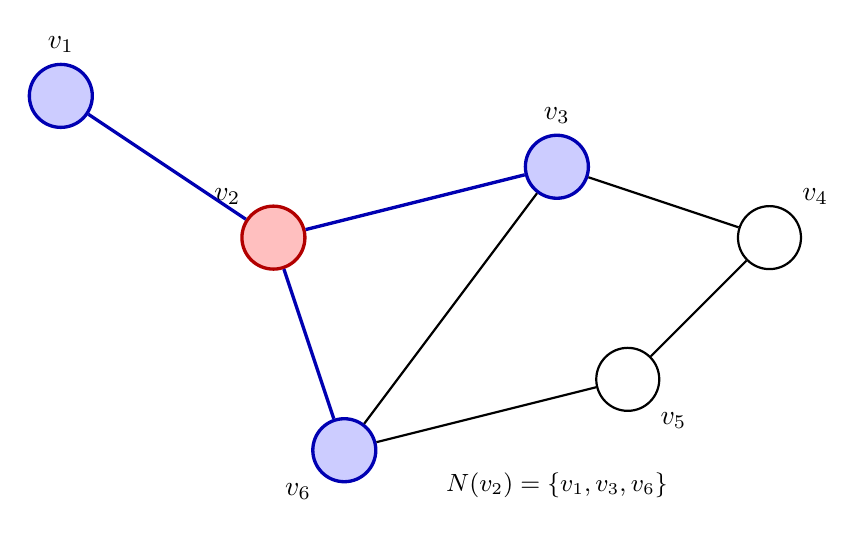
\begin{tikzpicture}[
        scale=0.9,
        vertex/.style={
            circle,
            draw=black,
            fill=white,
            thick,
            minimum size=8mm,
            inner sep=0pt,
            font=\small
        },
        neighbor/.style={
            vertex,
            draw=blue!70!black,
            fill=blue!20,
            very thick
        },
        selected/.style={
            vertex,
            draw=red!70!black,
            fill=red!25,
            very thick
        }
    ]

    % Vértices
    \node[neighbor,label=above:$v_1$] 
        (n1) at (1,10) {};

    \node[selected,label=above left:$v_2$] 
        (n2) at (4,8) {};

    \node[neighbor,label=above:$v_3$] 
        (n3) at (8,9) {};

    \node[vertex,label=above right:$v_4$] 
        (n4) at (11,8) {};

    \node[vertex,label=below right:$v_5$] 
        (n5) at (9,6) {};

    \node[neighbor,label=below left:$v_6$] 
        (n6) at (5,5) {};

    % Aristas pertenecientes al vecindario de v_2
    \draw[blue!70!black, very thick] (n1) -- (n2);
    \draw[blue!70!black, very thick] (n2) -- (n3);
    \draw[blue!70!black, very thick] (n2) -- (n6);

    % Aristas restantes
    \draw[thick] (n3) -- (n4);
    \draw[thick] (n4) -- (n5);
    \draw[thick] (n5) -- (n6);
    \draw[thick] (n6) -- (n3);

    % Leyenda del vecindario
    \node[
        draw=none,
        fill=none,
        rectangle,
        font=\small,
        align=left
    ] at (8,4.5) {$N(v_2)=\{v_1,v_3,v_6\}$};

    \end{tikzpicture}

    \caption{Vecindario del vértice $v_2$ en la gráfica $G$. 
    \\El vecindario resultante es $N(v_2)=\{v_1,v_3,v_6\}$}
    \label{fig:vecindario-v2}
\end{figure}


Otra de las definiciones que sirven tanto para caracterizar así como dar importancia a los nodos de una gráfica es el \textbf{grado de un vértice}. Así, está noción nos permite cuantificar la conectividad de cada vértice dentro de la gráfica, proporcionando información sobre su estructura y las relaciones entre los vértices. 

\begin{definition}[Grado de un vértice]
    El \textbf{grado} de $v$ es el numero de sus vecinos.
    \begin{center}
        $d_{G}(v)$ = $|N_G(v)|$.
    \end{center}  
\end{definition}

De la definición anterior podemos notar que para cualquier vértice $v$, podría suceder que $v$ no tenga vecinos o por el otro lado que el resto de los vértices de $G$ sean sus vecinos, recordando que $v$ no puede ser vecino de sí mismo. Así, se tiene que:
    \begin{center}
        0 $\leq$ $d_G(v)$ $\leq$ $n-1$
    \end{center} 
    donde $n$ es el orden la gráfica $G$.

    \begin{definition}[Vértice aislado]

    Cuando $d_G(v)$= 0 decimos que $v$ es un vértice aislado.
    \end{definition}
    
    \noindent Dada una gráfica $G = (V,E)$ con $V(G) = \{v_1,...,v_n\}$ sabemos que el conjunto:
    \[\{d_G(v_1),.\hspace{1pt} . \hspace{1pt}.\hspace{1pt},d_G(v_n)\}\]
    Es un conjunto finito de números naturales pues el conjunto V(G) lo es, entonces de esta forma podemos definir a $\delta(G)$ como el grado mínimo de G y $\Delta(G)$ como el grado máximo de G.

    \begin{definition}[Grado mínimo y grado máximo]
    Sea $G = (V,E)$ una gráfica simple, tenemos que;
    \begin{enumerate}
        \item  $\delta(G)$ = $min\{d_G(v_1),.\hspace{1pt}.\hspace{1pt}.\hspace{1pt},d_G(v_n)\}$ es el grado mínimo de $G$.
        \item $\Delta(G)$ = $max\{d_G(v_1),.\hspace{1pt}.\hspace{1pt}.\hspace{1pt},d_G(v_n)\}$ es el grado máximo de $G$.
    \end{enumerate}      
    \end{definition}

    \noindent Para la gráfica de la figura \ref{fig:G} tenemos que $\delta(G)$ = 1 y que $\Delta(G)$ = 3.

\begin{proposition}
Dada una gráfica $G$, tenemos que
\[\delta(G) \leq d(G) \leq \Delta(G).\]
    
\end{proposition}

\begin{proof}
    Sabemos que, por definición de grado mínimo y máximo, para todo $v \in V(G)$ se cumple que $\delta(G) \leq d_G(v) \leq \Delta(G)$. Sumando sobre todos los vértices:

    \[
    \sum_{v \in V(G)} \delta(G) \leq \sum_{v \in V(G)} d_G(v) \leq \sum_{v \in V(G)} \Delta(G)
    \]

    Como $\delta(G)$ y $\Delta(G)$ son constantes respecto a la suma, esto se puede escribir como:

    \[
    \nu_G \cdot \delta(G) \leq \sum_{v \in V(G)} d_G(v) \leq \nu_G \cdot \Delta(G)
    \]

    Dividiendo entre $\nu_G$ en toda la desigualdad, obtenemos:

    \[
    \delta(G) \leq \frac{1}{\nu_G} \sum_{v \in V(G)} d_G(v) \leq \Delta(G)
    \]

    Por definición, el término central es el grado promedio $d(G)$, así que finalmente:

    \[
    \delta(G) \leq d(G) \leq \Delta(G)
    \]
\end{proof}


\subsection{Representación de gráficas}

Existen diversas formas de representar gráficas, podemos encontrarlas en su forma visual como la de la figura \ref{fig:G}, o bien podemos encontrarlas en su forma matricial conocida como \textbf{matriz de adyacencia}. 
La matriz de adyacencia es una representación matricial de una gráfica que permite identificar rápidamente la conexión entre los vértices. 
En esta matriz, las filas y columnas representan los vértices de la gráfica, y los elementos de la matriz indican si existe una arista entre los vértices correspondientes.
A continuación, definiremos formalmente la matriz de adyacencia de una gráfica simple y presentaremos un ejemplo para ilustrar su uso.

\begin{definition}[Matriz de Adyacencia]
    Sea $V_G = \{v_1,...,v_n\}$ ordenado. 
    La matriz de adyacencia $\mathbf{A}$ de $\mathbf{G}$ está definida cómo \begin{center}
        $\mathbf{A}(\mathbf{G})$ = $\left[a_{ij}\right]$
    \end{center}
    donde:
    \begin{center}
        $a_{ij}$=$\left\lbrace\begin{array}{c} 1~si~v_iv_j \in \mathbf{E_G} \\0~si~no \end{array}\right.$
    \end{center}
\end{definition}

\begin{example}
    La matriz de adyacencia de la figura \ref{fig:G} quedaría de la siguiente forma:
\begin{center}
\begin{equation}
A(G) =
\begin{pmatrix}
0 & 1 & 0 & 0 & 0 & 0\\
1 & 0 & 1 & 0 & 0 & 1\\
0 & 1 & 0 & 1 & 0 & 1\\
0 & 0 & 1 & 0 & 1 & 0\\
0 & 0 & 0 & 1 & 0 & 1\\
0 & 1 & 1 & 0 & 1 & 0
\end{pmatrix}
\end{equation}
    
\end{center}
\end{example}
\noindent Notamos que la matriz de adyacencia es una matriz simétrica, ya que si $v_i$ y $v_j$ son vecinos entonces $v_j$ y $v_i$ también lo son, por lo tanto $a_{ij}$ = $a_{ji}$.
\noindent Además, notamos que la diagonal principal de la matriz de adyacencia es cero, ya que no existe una arista que conecte un vértice consigo mismo en una gráfica simple.

Una alternativa que mejora notablemente la optimización de memoria es la representación de gráficas mediante listas de adyacencia. Este modelo asocia a cada vértice una colección de sus nodos colindantes, lo que permite un acceso más rápido a la información de la conexiones entre los vértices al prescindir de una matriz completa.

\begin{definition}[Lista de adyacencia]
    Sea $G = (V,E)$ una gráfica simple. La \textbf{lista de adyacencia} de $G$ es un conjunto de listas $\{L_v\}_{v \in V}$ donde cada lista $L_v$ contiene los vértices adyacentes a $v$. Es decir, para cada vértice $v \in V$, tenemos:
    \begin{center}
        $L_v = \{u \in V \mid vu \in E\}$
    \end{center}
\end{definition}
\noindent En la figura \ref{fig:G}, la lista de adyacencia sería:
\begin{example}
    Sea $G = (V,E)$ la gráfica de la figura \ref{fig:G}, entonces la lista de adyacencia de $G$ sería:
    \begin{center}
        \begin{tabular}{c|c}
            Vértice & Lista de adyacencia \\
            \hline
            $v_1$ & $\{v_2\}$ \\
            $v_2$ & $\{v_1, v_3, v_6\}$ \\
            $v_3$ & $\{v_2, v_4, v_6\}$ \\
            $v_4$ & $\{v_3, v_5\}$ \\
            $v_5$ & $\{v_4, v_6\}$ \\
            $v_6$ & $\{v_2, v_3, v_5\}$
        \end{tabular}
    \end{center}
\end{example}

\subsection{Subgráficas}

Debido a los métodos que se utilizarán más adelante en el estudio de los objetos y debido al gran número de datos a procesar, es necesario introducir conceptos que se pueden emplear para el estudio local de las gráficas. De este modo introduciremos el concepto de subgráfica. 
\begin{definition}[Subgráfica]
Sea $G = (V,E)$ una gráfica simple. Una subgráfica de $G$ es una gráfica $H = (V_H,E_H)$ tal que: $\subseteq G $, si $V(H) \subseteq  V(G)$ Y $E(H) \subseteq E(G)$.
\end{definition}

\begin{figure}[H]
    \centering
    \begin{tikzpicture}[
        scale=0.9,
        every node/.style={
            circle,
            draw=black,
            fill=white,
            thick,
            minimum size=8mm,
            inner sep=0pt,
            font=\small
        }
    ]
    
    % Vértices
    \node[label=above:$v_1$]      (n1) at (1,10) {};
    \node[label=above left:$v_2$] (n2) at (4,8)  {};
    \node[label=above:$v_3$]      (n3) at (8,9)  {};
    \node[label=above right:$v_4$](n4) at (11,8) {};
    \node[label=below left:$v_6$] (n6) at (5,5)  {};

    % Aristas
    \draw[thick] (n1) -- (n2);
    \draw[thick] (n2) -- (n3);
    \draw[thick] (n3) -- (n4);
    \draw[thick] (n3) -- (n6);
    \draw[thick] (n6) -- (n2);

    \end{tikzpicture}
    \caption{Ejemplo de subgráfica de $G$.}
    \label{fig:SG}
\end{figure}

\begin{definition}
    Sea $G$ una gráfica simple y $H$ una subgráfica de $G$. 
    Decimos que una subgráfica $H \subseteq G$ abarca $G$ (y $H$ es una subgráfica generadora de $G$) si cada vértice de $G$ está en $H$, i.e $V(H) = V(G)$\\
\end{definition}

\begin{figure}[H]
    \centering
    \begin{tikzpicture}[
        scale=0.9,
        every node/.style={
            circle,
            draw=black,
            fill=white,
            thick,
            minimum size=8mm,
            inner sep=0pt,
            font=\small
        }
    ]
    
    % Vértices
    \node[label=above:$v_1$]       (n1) at (1,10)  {};
    \node[label=above left:$v_2$]  (n2) at (4,8)   {};
    \node[label=above:$v_3$]       (n3) at (8,9)   {};
    \node[label=above right:$v_4$] (n4) at (11,8)  {};
    \node[label=below right:$v_5$] (n5) at (9,6)   {};
    \node[label=below left:$v_6$]  (n6) at (5,5)   {};

    % Aristas
    \draw[thick] (n1) -- (n2);
    \draw[thick] (n2) -- (n3);
    \draw[thick] (n6) -- (n2);
    \draw[thick] (n6) -- (n5);
    \draw[thick] (n5) -- (n4);

    \end{tikzpicture}
    \caption{Ejemplo de una gráfica $H$ que abarca a $G$.}
    \label{fig:GA}
\end{figure}

\begin{definition} 
    Sea $G$ una gráfica simple.
    Decimos que una subgráfica $H \subseteq G$, es una subgráfica inducida, si $E(H) = E(G) \cap E(V_H)$. En este caso $H$ es inducido por el conjunto $V(H)$ de vértices.
\end{definition}
\noindent En otras palabras, una subgráfica inducida es aquella que contiene todas las aristas de $G$ que conectan los vértices de $H$. Esto significa que si dos vértices en $H$ están conectados por una arista en $G$, entonces esa arista también estará presente en $H$.

\begin{figure}[H]
    \centering
    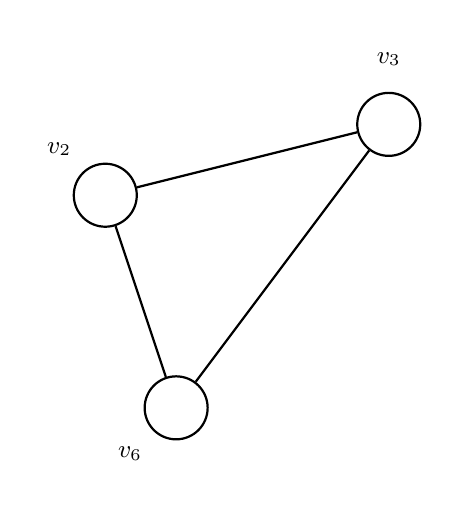
\begin{tikzpicture}[
        scale=0.9,
        every node/.style={
            circle,
            draw=black,
            fill=white,
            thick,
            minimum size=8mm,
            inner sep=0pt,
            font=\small
        }
    ]
    
    % Vértices
    \node[label=above left:$v_2$] (n2) at (4,8) {};
    \node[label=above:$v_3$]      (n3) at (8,9) {};
    \node[label=below left:$v_6$] (n6) at (5,5) {};

    % Aristas
    \draw[thick] (n2) -- (n3);
    \draw[thick] (n6) -- (n2);
    \draw[thick] (n3) -- (n6);

    \end{tikzpicture}
    \caption{Ejemplo de una gráfica inducida.}
    \label{fig:GI}
\end{figure}

 \subsection{Caminos y ciclos}
 Uno de los conceptos fundamentales que se introducirán y además se implementarán en la creación de los algoritmos de la sección final es el concepto de caminos, este concepto se utilizará cómo herrramienta para el estudio del recorrido de la gráfica completa.

 \begin{definition}[Camino, ciclo y caminos cerrados]
    
     Sea $e_i = u_iu_{i+1} \in E(G)$ aristas de $G$ para $i \in \{1,...,k\}$. \\
     Un camino es una gráfica no vacía $W = (V,E)$ de la forma;
     \begin{center}
         $V = \{u_0,u_1,...,u_k,u_{k+1}\}$ \hspace{5pt} $E= \{e_0,e_1,...,e_k\}$
     \end{center}
     donde:
     $u_i$ es adyacente a $u_{i+1}$
     para todo $i \in \{1,...,k\}$.\\
     Además:
     \begin{enumerate}
         \item $W$ es \textbf{cerrado}, si $u_0 =u_{k+1}$.
         \item $W$ es un \textbf{camino}, si $u_i \neq u_j$, para todo $i \neq j$.
         \item W es un \textbf{ciclo}, si es cerrado y $u_i \neq u_j$ para $i \neq j$ excepto para $u_1 = u_{k+1}$
         
     \end{enumerate}
     
     Además, el número $l(W)$ es el tamaño o longitud del camino y está dado por $l(W)=|E(W)|$
 \end{definition}

\begin{figure}[H]
    \centering
    
    % Ejemplo de camino
    \begin{minipage}{0.45\textwidth}
        \centering
        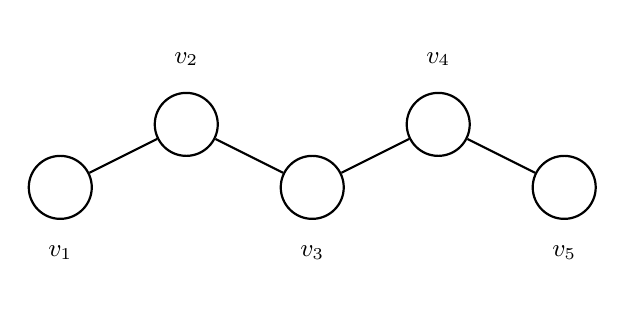
\begin{tikzpicture}[
            scale=0.8,
            every node/.style={
                circle,
                draw=black,
                fill=white,
                thick,
                minimum size=8mm,
                inner sep=0pt,
                font=\small
            }
        ]
        
        % Vértices
        \node[label=below:$v_1$]       (n1) at (0,0) {};
        \node[label=above:$v_2$]       (n2) at (2,1) {};
        \node[label=below:$v_3$]       (n3) at (4,0) {};
        \node[label=above:$v_4$]       (n4) at (6,1) {};
        \node[label=below:$v_5$]       (n5) at (8,0) {};

        % Aristas
        \draw[thick] (n1) -- (n2);
        \draw[thick] (n2) -- (n3);
        \draw[thick] (n3) -- (n4);
        \draw[thick] (n4) -- (n5);

        \end{tikzpicture}
        \caption{Ejemplo de un camino.}
        \label{fig:camino}
    \end{minipage}
    \hfill
    % Ejemplo de ciclo
    \begin{minipage}{0.45\textwidth}
        \centering
        \begin{tikzpicture}[
            scale=0.8,
            every node/.style={
                circle,
                draw=black,
                fill=white,
                thick,
                minimum size=8mm,
                inner sep=0pt,
                font=\small
            }
        ]

        % Vértices
        \node[label=left:$v_1$]  (n1) at (0,0) {};
        \node[label=above:$v_2$] (n2) at (2,2) {};
        \node[label=right:$v_3$] (n3) at (4,0) {};
        \node[label=below:$v_4$] (n4) at (2,-2) {};

        % Aristas
        \draw[thick] (n1) -- (n2);
        \draw[thick] (n2) -- (n3);
        \draw[thick] (n3) -- (n4);
        \draw[thick] (n4) -- (n1);

        \end{tikzpicture}
        \caption{Ejemplo de un ciclo.}
        \label{fig:ciclo}
    \end{minipage}
\end{figure}

 \subsection{Árboles}
 Una forma de reducir el número de vértices sin que la gráfica pierda gran parte de su información, es mediante el estudio de los árboles, veremos su definición y los conceptos más importantes relacionados con el estudio de estas estructuras.

  \begin{definition}[Gráfica conexa]
     Una gráfica $G=(V,G)$ es conexa si para cualquier par de vértices $u \hspace{5pt} y \hspace{5pt} v$ de G si existe un camino que inicia en $u$ y termina en $v$ 
\end{definition}

\begin{figure}[H]
    \centering
    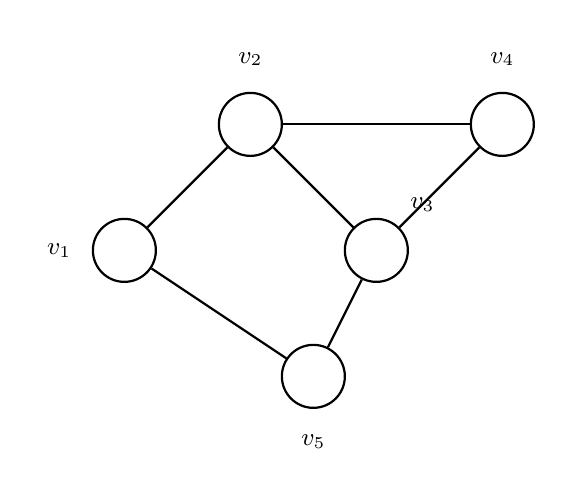
\begin{tikzpicture}[
        scale=0.8,
        every node/.style={
            circle,
            draw=black,
            fill=white,
            thick,
            minimum size=8mm,
            inner sep=0pt,
            font=\small
        }
    ]

    % Vértices
    \node[label=left:$v_1$]        (n1) at (0,0)  {};
    \node[label=above:$v_2$]       (n2) at (2,2)  {};
    \node[label=above right:$v_3$] (n3) at (4,0)  {};
    \node[label=above:$v_4$]       (n4) at (6,2)  {};
    \node[label=below:$v_5$]       (n5) at (3,-2) {};

    % Aristas
    \draw[thick] (n1) -- (n2);
    \draw[thick] (n2) -- (n3);
    \draw[thick] (n3) -- (n4);
    \draw[thick] (n3) -- (n5);
    \draw[thick] (n5) -- (n1);
    \draw[thick] (n2) -- (n4);

    \end{tikzpicture}
    \caption{Ejemplo de una gráfica conexa.}
    \label{fig:conexa}
\end{figure}

 Notamos que una gráfica $G$ es conexa si y sólo si tiene una única componente conexa, es decir, si no se puede dividir en subgráficas conexas más pequeñas. En caso contrario, si $G$ no es conexa, entonces se puede dividir en múltiples componentes conexas, cada una de las cuales es maximal con respecto a la propiedad de ser conexa.
 \begin{definition}[Puente]
 Dada un gráfica $G$ conexa y una arista $e \in E_G$. Decimos que \textbf{e} es un puente de la gráfica $G$, si $G - e$ es disconexa.
 \end{definition}

 \begin{figure}[H]
    \centering
    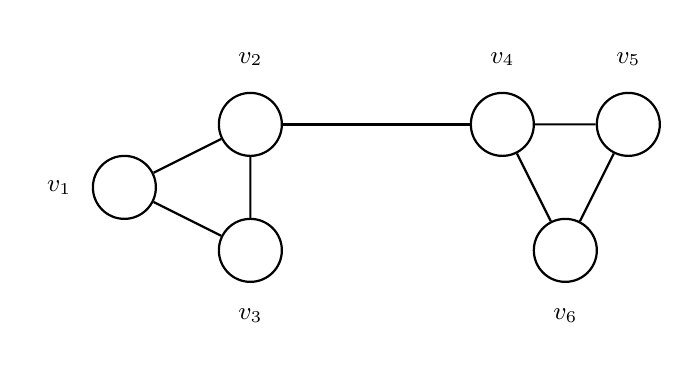
\begin{tikzpicture}[
        scale=0.8,
        every node/.style={
            circle,
            draw=black,
            fill=white,
            thick,
            minimum size=8mm,
            inner sep=0pt,
            font=\small
        }
    ]
    
    % Primer componente triangular
    \node[label=left:$v_1$]         (a1) at (0,0)  {};
    \node[label=above:$v_2$]        (a2) at (2,1)  {};
    \node[label=below:$v_3$]        (a3) at (2,-1) {};

    \draw[thick] (a1) -- (a2);
    \draw[thick] (a1) -- (a3);
    \draw[thick] (a2) -- (a3);

    % Segundo componente triangular
    \node[label=above:$v_4$]        (b1) at (6,1)  {};
    \node[label=above:$v_5$]        (b2) at (8,1)  {};
    \node[label=below:$v_6$]        (b3) at (7,-1) {};

    \draw[thick] (b1) -- (b2);
    \draw[thick] (b2) -- (b3);
    \draw[thick] (b3) -- (b1);

    % Puente
    \draw[very thick] (a2) -- (b1);

    \end{tikzpicture}
    \caption{Ejemplo de una gráfica con un puente (arista de corte).}
    \label{fig:puente}
\end{figure}
 
En la figura \ref{fig:puente} notamos que la arista $de$ es un puente, ya que si la eliminamos, la gráfica resultante se vuelve disconexa, separando los vértices $a$, $b$ y $c$ de los vértices $d$, $e$ y $f$.
 
 \begin{proposition}
     Sea una gráfica $G$.
     Un vértice $e \in E(G)$ es un puente de $G$ si y sólo sí $e$ no está en ningún ciclo de $G$.
 \end{proposition}
 
 \begin{proof}

 Primero notemos que $e=uv$ es un puente sí y sólo sí $u$, $v$ pertenecen a diferentes componentes conexas de $G-e$, pues de lo contrario implicaría que existe un camino que conecta a $u$ con $v$ lo cual sería una contradicción ya que $G-e$ es disconexo.
 
     ($\Rightarrow$) Por contrapositiva, Supongamos que existe un ciclo de $G$ que contiene a $e$, entonces existe un camino tal que $C = \{u_0=u,v,...,u_{k+1}=u\}$.
     De aquí, notamos que en $G-e$ existe un camino $C' = \{v_0=v,...,v_{k+1} = u\}$,entonces existe un camino alterno que conecta a $u$ con $v$ lo cual implica que $G-e$ es conexa. Por tanto $e=uv$ no es puente.
     \newline
     ($\Leftarrow$) Supongamos que $e=uv$ no es puente, por la observación hecha al inicio esto implica que $u$,$v$ pertenecen a la misma componente conexa de $G-e$.Entonces existe un camino que $C=\{v_0=v,...,v_{k+1} = u\}$ conecta a $v$ con $u$, de ahí notamos que $eC$ es un ciclo pues $eC = \{u,v_0=v,...,v_{k+1}=u\}$.
\end{proof}
 

 \begin{definition}[Gráfica acíclica]
     Una gráfica es llamada acíclica si no contiene ciclos.
 \end{definition}


 \begin{definition}[Árbol]
  Un árbol es una gráfica acíclica y conexa.
 \end{definition}
\begin{figure}[H]
    \centering
    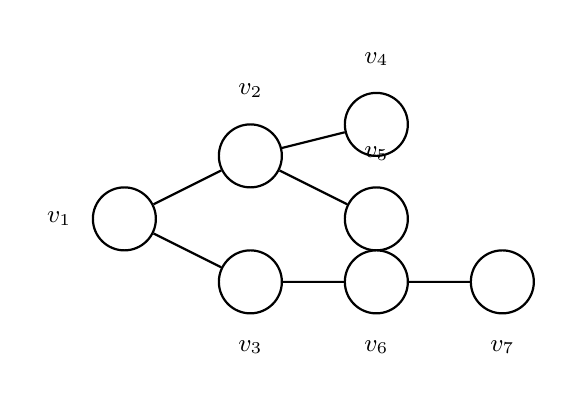
\begin{tikzpicture}[
        scale=0.8,
        every node/.style={
            circle,
            draw=black,
            fill=white,
            thick,
            minimum size=8mm,
            inner sep=0pt,
            font=\small
        }
    ]
    
    % Vértices del árbol
    \node[label=left:$v_1$]        (a) at (0,0)   {};
    \node[label=above:$v_2$]       (b) at (2,1)   {};
    \node[label=below:$v_3$]       (c) at (2,-1)  {};
    \node[label=above:$v_4$]       (d) at (4,1.5) {};
    \node[label=above:$v_5$]       (e) at (4,0) {};
    \node[label=below:$v_6$]       (f) at (4,-1)  {};
    \node[label=below:$v_7$]       (g) at (6,-1)  {};

    % Aristas del árbol
    \draw[thick] (a) -- (b);
    \draw[thick] (a) -- (c);
    \draw[thick] (b) -- (d);
    \draw[thick] (b) -- (e);
    \draw[thick] (c) -- (f);
    \draw[thick] (f) -- (g);

    \end{tikzpicture}
    \caption{Ejemplo de una gráfica acíclica (un árbol).}
    \label{fig:aciclica}
\end{figure}

 
 De la \textbf{Proposición 2.2} y la \textbf{Definición 22} se deriva el siguiente corolario.
 
 \begin{corollary}
     Una gráfica conexa es un árbol sí y sólo sí todas sus aristas son puentes.
 \end{corollary}
\noindent Notamos que un árbol es una gráfica conexa y acíclica, además de que todas sus aristas son puentes. Esto implica que si eliminamos cualquier arista de un árbol, la gráfica resultante se vuelve disconexa, lo cual es una propiedad clave de los árboles.
 \begin{teorema}
 Los siguientes enunciados son equivalentes:
  \begin{enumerate}
         \item $T$ es un arbol
         \item Cualesquiera dos vértices estan conectados en $T$ por un único camino.
         \item $T$ es aciclico y $\varepsilon_T = \nu_T - 1$
\end{enumerate}
     
 \end{teorema}
 
\begin{proof}
Sea \boldmath{$\nu_T$} = \textbf{n}, Si n=1 el teorema es trivial,así que supongamos para n $\geq$ 2.\\

    (1) $\Rightarrow$ (2) Supongamos que $T$ es un árbol. Sean $u$ y $v$ dos vértices de $T$ y por contradicción supongamos que existen dos caminos $P$ y $Q$ tales que conectan a \textbf{u} y \textbf{v}. Sin pérdida de generalidad supongamos que $l(P) > l(Q)$. Entonces existe al menos una arista \textbf{e} que está en $P$ pero no está en $Q$. Por \textbf{Corolario 2} sabemos que cada arista de $T$ es un puente. Y por lo visto anteriormente entonces \textbf{u} y \textbf{v} están en diferentes componentes conexas de $T-e$.Pero notamos que por el camino $Q$ siguen estando conectados. Lo cual es una contradicción ya que implicaria que \textbf{u} y \textbf{v} no estén en diferentes componentes conexas.\\

    (2) $\Rightarrow$ (3) Esta implicación la probaremos por inducción sobre \textbf{n}.
\\ Para $n=2$.
Sabemos que no existen componentes disconexas pues cualesquiera dos vértices están conectados por un camino, por lo cual $\varepsilon_T = 1 = 2-1= \nu_T -1$.
\\Supongamos que la afirmación se cumple para los valores menores a \textbf{n} y probemos para \textbf{n}.\\
Sea \textbf{P} el máximo camino en $T$ entre \textbf{u} y \textbf{v}, es decir que no existen aristas $e$ tales que $eP$  o $Pe$ sean caminos. De ahí que $d_T(v) = 1$.Si $uw \in E(T)$ entonces $w \in P$.
Ahora notamos que la subgráfica $T-v$ está conectada por un único camino $P'$ , además notamos que $l(P)$ es a lo más $n$ y cómo $l(P)>l(P')$ entonces $l(P') \leq n-1$ dado que la subgráfica $T-v$ esta conectada por un único camino (Pues $T$ lo está) y por hipotésis de inducción tenemos que:\\
\[\varepsilon_{T-v} = \nu_{T-v} - 1 = (n-1)-1 = n-2\]

Y de ahí que:
\[\varepsilon_T = \varepsilon_{T-v} + 1 = n-1\] \\
(3) $\Rightarrow$ (1) Supongamos (3). Basta con probar que $T$ es conexo.
Sean $T_i=(V_i,E_i)$ componentes conexos de $T$ para $i \in \{1,...k\}$. Sabemos que $T$ es acíclico,por lo tanto sus componentes conexos $T_i$ también los son por tanto $|E_i| = |V_i| - 1$.
Notemos que:
\begin{center}
    $\nu_T$ = $\sum_{i=1}^{k} |V_i|$
        ,
        $\varepsilon_T$ = $\sum_{i=1}^{k} |E_i|$
\end{center}
Entonces:

\begin{center}
    \[n-1 = \varepsilon_T = \sum_{i=1}^{k} (|V_i| - 1)= \sum_{i=1}^{k}|V_i| - k = n-k\] 
    \[\therefore k =1\]
\end{center}
Lo cual quiere decir que $T$ es un sólo componente conexo, por lo tanto $T$ es un árbol.    
\end{proof}

\begin{definition}[Árbol generador]
    Dada una gráfica conexa $G$ una subgráfica $T$ de $G$ es un subárbol generado de $G$ si satisface que;

    \begin{enumerate}
        \item $T$ es una subgráfica generadora de $G$ y
        \item $T$ es un árbol.
    \end{enumerate}
\end{definition}
\begin{teorema}
    Cada gráfica conexa contiene un árbol generador.
\end{teorema}
\begin{proof}
    Sea $H\subset G$ la mínima gráfica generadora conexa de $G$, es decir $H-e$ es disconexa para todo $e \in E(H)$.
    Esta gráfica es obtenida de $G$ removiendo todas las aristas que no son puentes:
    \begin{enumerate}
        \item Hacemos $H_0 = G$.
        \item Para $i \geq 0$ sea $H_{i+1} = H_i - e_i$ donde $e$ no es un puente de $H_i$. Como $e_i$ no es un puente $H_{i+1}$ es una subgráfica generadora y conexa de $H_i$ y por lo tanto de $G$.
        \item De este forma hacemos $H = H_k$ cuando sólo quedan puentes en la subgráfica.
        Y por el \textbf{Coroloraio2} $H$ es un árbol.
    \end{enumerate}
\end{proof}

\begin{definition}[Árbol generador mínimo]
    
    Un árbol generador mínimo es un árbol generador tal que la suma de los pesos de sus aristas es la mínima posible, es decir.
\begin{center}
    $w(T) = \sum_{(u,v) \in T} min\{w(u,v)\}$
\end{center}
Donde $w(u,v)$ es el peso que hay entre el vértice $u$ y la arista $v$.
\end{definition}

Con lo definido hemos establecido una base sólida para el estudio de nuestras estructuras de interés. Al abordar formalmente las superficies y su discretización a través de complejos simpliciales y así al traducirlos nuevamente a gráficas podemos garantizar que los algoritmos que desarrollaremos posteriormente operen de manera eficiente y precisa.
De la mano de estos conceptos, podemos dar el siguiente paso e introducir en el siguiente capítulo el paradigma de las rede neuronales, que nos permitirá abordar problemas complejos de manera más efectiva y con un enfoque basado en el aprendizaje automático.Detallaremos como esta intersección nos proporciona las herramientas algorítmixas necesarias para abordar problemas de optimización y análisis de datos en el contexto de las gráficas y sus aplicaciones en diversas áreas.
